\section{Understanding Events}
Understanding events is a fundamental prerequisite for deeper semantic 
analysis of language.  We introduce the problem of automatic anomalous event
detection
in this paper and propose a novel event model that can learn to differentiate
between normal
and anomalous events.  We generally define anomalous events as those that are
unusual compared
to the general state of affairs and might invoke surprise when reported.  For
example, given the event mention in the 
following sentence 
\begin{itemize}
 \item[] \textit{Man recovering after being shot by his dog.}
\end{itemize}
one might think it is strange because \textit{dogs} are not expected
to shoot \textit{men}.  But the mentions
\begin{itemize}
 \item[] \textit{Man recovering after being shot by cops.}
 \item[] \textit{Man recovering after being bitten by a dog.}
\end{itemize}
are not as unusual as the previous one.  While all three sentences are equally
valid syntactically, and it is not unclear what any of them means, it 
is our knowledge about the role fillers 
---both individually and specifically in combination---  
that enables us to 
differentiate between normal and anomalous events.  Hence we hypothesize that
\emph{anomaly is a result of unexpected or 
unusual combination of semantic role fillers}.  Given this idea, an automatic
anomaly detection algorithm has to encode
the goodness of semantic role filler coherence.  


It has to be noted that event level anomaly is not the same as semantic incoherence.
An event constructed by randomly choosing words to form each of the semantic arguments
is not anomalous since we cannot argue whether the event is normal or anomalous when
it is unclear what the event means.  Hence, we define anomalous events to be the 
sub class of those that are semantically coherent, but are unusual only based on 
real world knowledge.

Automatic anomalous event detection is a hard problem since
determining what a good combination of role fillers
requires deep semantic and pragmatic knowledge.  
Moreover, manual judgment of anomaly itself may be difficult and people often
may not agree with each other in this
regard.  We describe the difficulty in human judgment in greater detail in
Section~\ref{sec:annot}.  
Automatic detection of anomaly requires encoding complex information, which has 
to be composed from the semantics of the individual words in the sentence.  A 
fundamental problem in doing so is the sparsity in semantic space due to 
the discrete representations of meaning of words. 

\section{Background: Selectional Preference and Thematic Fit}
Selectional preference, a notion introduced by \cite{wilks1973preference}, refers to the phenomenon 
of the predicate and the fillers of its arguments
affecting the likelihood of fillers of other arguments.  Thus the idea is that predicate and the role fillers 
``prefer'' some fillers for other roles.  For example, given that the predicate is \textit{writes}, the 
agent \textit{author} prefers the patient \textit{book}, while the agent \textit{programmer} prefers the 
patient \textit{code}.  This idea is used by \cite{elman2009meaning}, and is very similar to the 
role-filler composition that we use for anomaly detection.

\cite{erk2010flexible} also model selectional preferences using vector spaces.  They measure the 
goodness of the fit of a noun with a verb in terms of the similarity between the vector of the noun and 
some ``exemplar'' nouns taken by the verb in the same argument role.  \cite{baroni2010distributional} 
also measure selectional preference similarly, but instead of exemplar nouns, they calculate a 
prototype vector for that role based on the vectors of the most common nouns occurring in that 
role for the given verb.  \cite{lenci2011composing} builds on this work and models the phenomenon
that the expectations of the verb or its role-fillers change dynamically given other role fillers.

\section{Data}
We crawl 3684 ``weird news'' headlines available publicly 
on the website of NBC
news\footnote{\url{
http://www.nbcnews.com/html/msnbc/3027113/3032524/4429950/4429950_1.html}}, 
such as the following: 
\begin{itemize}
 \item \textit{India weaponizes world's hottest chili.}
 \item \textit{Man recovering after being shot by his dog.}
 \item \textit{Thai snake charmer puckers up to 19 cobras.}
\end{itemize}
We assume that the events extracted from this source, called NBC Weird Events
(NWE) henceforth, are
anomalous for training.  NWE contains 4271 events extracted using 
SENNA's SRL.  We use 3771 of those events as our negative training data. 
Similarly, we extract events also from
headlines in the AFE section of Gigaword, called Gigaword Events (GWE)
henceforth.  We assume these events are normal.
To use as positive examples for training event composition, we sample roughly
the same number of events from 
GWE as our negative examples from NWE. From the two sets, we uniformly sample 1003 events
as the test set and validate the labels by getting crowd-sourced annotations.

\subsection{Annotation}
\label{sec:annot}
We posted the annotation of the test set containing 1003 events as
Human Intelligence Tasks (HIT) on Amazon Mechanical Turk (AMT).
We broke the task into 20 HITs and asked the workers to select one of the 
four options - \textit{highly unusual}, \textit{strange}, \textit{normal} and 
\textit{cannot say} for each event.  We asked them to select \textit{highly
unusual} when the 
event seems too strange to be true, \textit{strange} if it seems unusual but 
still plausible, and \textit{cannot say} only if the information present in the 
event is not sufficient to make a decision.

\begin{table}
\begin{center}
  \begin{tabular}[c]{|c|c|}
 \hline
  Total number of annotators & 22\\
  \hline
  \textit{Normal} annotations & 56.3\% \\
  \hline
  \textit{Strange} annotations & 28.6\% \\
  \hline
  \textit{Highly unusual} annotations & 10.3\% \\
  \hline
  \textit{Cannot Say} annotations & 4.8\% \\
  \hline
  Avg. events annotated per worker & 344 \\
  \hline
  4-way Inter annotator agreement ($\alpha$) & 0.34 \\
  \hline
  3-way Inter annotator agreement ($\alpha$) & 0.56 \\
  \hline
  \end{tabular}
\end{center}
 \caption{Annotation Statistics}
 \label{table:annot}
\end{table}
Table~\ref{table:annot} shows some statistics of the annotation task.  We
computed the Inter Annotator
Agreement (IAA) in terms of Kripendorff's alpha \cite{krippendorff1980content}. 
The advantage of using this
measure instead of the more popular Kappa is that the former can deal with
missing information, which is the case with
our task since annotators work on different overlapping subsets of the test set.
 The 4-way IAA shown in the table 
corresponds to agreement over the original 4-way decision (including
\textit{cannot say}' while the 3-way IAA is measured after merging the 
\textit{highly unusual} and \textit{strange} decisions.  

Additionally we used
MACE \cite{hovy2013learning} to assess the quality of 
annotation.  MACE models the annotation task as a generative process of
producing the observed labels conditioned on the 
true labels and the competence of the annotators, and predicts both the latent
variables.  The average of competence of annotators, 
a value that ranges from 0 to 1, for our task is 0.49 for the 4-way decision and
0.59 for the 3-way decision.  

We generated
true label predictions produced by MACE, discard the events for which the
prediction remains to be \textit{cannot say}, and use the 
rest as the final labeled test set.  This left 949 events as our test dataset,
of which only 41\% of the labels are \textit{strange} or \textit{highly
unusual}.  It has to be noted that even though our test set 
has equal size samples from both NWE and GWE, the true distribution is not
uniform.

\subsection{Language Model Separability}
Given the annotations, we test to see if the
sentences corresponding to anomalous events can be separated from normal events by simpler 
features.  We build a n-gram language model from the training data set used for argument composition and 
measure the perplexity of the sentences in the test set.  Figure~\ref{fig:event_anomaly_ppl} shows
a comparison of the perplexity scores for different labels. If the n-gram features are enough 
to separate different classes of sentences, one would expect the sentences corresponding to 
\textit{strange} and \textit{highly unusual} labels to have higher perplexity ranges than \textit{normal}
sentences, because the language model is built from a dataset that is expected to have a distribution of
sentences where majority of them contain normal events.  As it can be seen in Figure~\ref{fig:event_anomaly_ppl}, 
except for a few outliers, most data points in all the categories are in similar perplexity ranges.
Hence, sentences with different labels cannot be separated based on an n-gram language model features.

\begin{figure}
  \begin{center}
  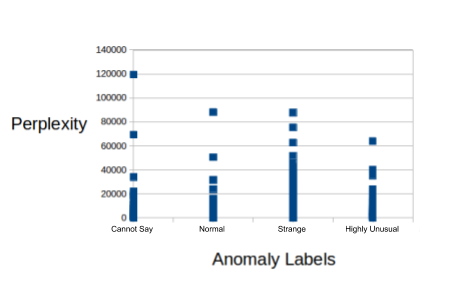
\includegraphics[width=3.5in]{figures/event_anomaly_lm_ppl.png}
  \caption{Comparison of perplexity scores for different labels for newswire headlines}
  \label{fig:event_anomaly_ppl}
  \end{center}
\end{figure}


\section{Model for Semantic Anomaly Detection}
We now describe our Neural Event Model (NEM) for encoding events. Events encoded using this model are then passed to a multi-layer perceptron
for making the anomaly decision. We define an event as the pair $(V, \textbf{A})$, where $V$
is a semantic verb\footnote{By semantic verb, we mean an action word whose
syntactic category is not necessarily a verb.  
For example, in \textit{Terrorist attacks on the World Trade Center..},
\textit{attacks} is not a verb but is still an 
action word.}, and $\textbf{A}$ is the set of its semantic arguments like agent,
patient, time, location, so on. Our aim
is to obtain a vector representation of the event that is composed from
representations of individual words, while explicitly guided by the semantic
role structure.
This representation can be understood as an embedding of the
event
in an event space.  

\subsection{Encoder}
Neural Event Model (NEM) is a kind of RNN
that is guided by a tree representation of events like the one shown in
Figure~\ref{fig:nem_event_tree}.  The edges 
connected to the root of the tree correspond to the verb and its semantic roles
(arguments).  All the other edges form binary sub-trees of arguments.  
\begin{figure}
  \begin{center}
  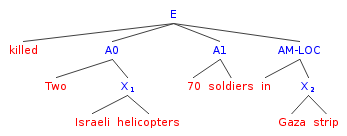
\includegraphics[width=4in]{figures/event_tree.png}
  \caption{Example of an event tree}
  \label{fig:nem_event_tree}
  \end{center}
 \end{figure}
NEM is a supervised model that learns to differentiate between anomalous and
normal events by 
classifying the event embeddings.  
The inputs to NEM are the semantic arguments, and the representations of words
in 
each argument.  We recursively compose the words in each argument to obtain
argument level
representations, which are then composed to obtain an event embedding. 

Intra-argument composition 
(called argument composition henceforth) is unsupervised, and we use contrastive
estimation 
to learn the parameters.  The structure of the binary tree backing
argument composition is determined dynamically, composing at each stage the two
nodes
which give the best composition score.  Inter-argument 
composition (called event composition henceforth) is supervised
and we use label error to learn the parameters.  Figure~\ref{fig:nem}
shows how NEM encodes the event shown in Figure~\ref{fig:nem_event_tree}.  The blue
boxes show argument composition 
and the red box shows event composition.  
\begin{figure}
  \begin{center}
  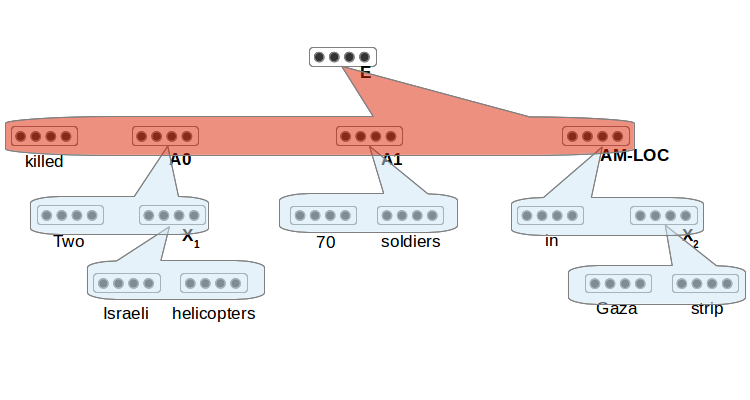
\includegraphics[width=4in]{figures/nem2.png}
  \caption{Neural Event Model: Encoding}
  \label{fig:nem}
  \end{center}
\end{figure}

\subsection{Training}
NEM is trained in two phases.  The first, argument composition is unsupervised 
while the second, event composition is supervised.
\subsubsection{Argument Composition}
An argument composition node takes inputs of dimensionality $2n$ and produces an
composed output representation
of dimensionality $n$ and a composition score.  Accordingly, we define the node
in terms of the parameters $\theta_{arg} = \{W_{arg} \in \mathbb{R}^{n \times 2n}; b_{arg}, S_{arg} \in
\mathbb{R}^{n \times 1}; V\}$
where $W_{arg}$, $b_{arg}$ and $S_{arg}$ are the composition weight, bias and
the scoring operators respectively 
as described previously, and $V$ is the set of representations of all the words
in the vocabulary.  
All nodes performing argument composition use the same parameters.  Training is
done in contrastive estimation fashion
and the objective is 
\begin{equation*}
 \argmin_{\theta_{arg}} J_{arg} = \argmin_{\theta_{arg}} max(0, 1-s+s_c)
\end{equation*}
where $s$ is the score of the composition of the entire argument produced by 
the root node of the argument, and $s_c$ is the score produced by randomly
replacing one of the words in the argument at a time. 
\subsubsection{Event Composition}
Event composition takes argument representations and produces the event
representation and label indicating whether the event is
normal or anomalous.  We define the event composition node in terms of the
parameters $\theta_{event} = \{W_{event} \in \mathbb{R}^{n \times kn}; b_{event},
L_{event} \in \mathbb{R}^{n \times 1}\}$
where $k$ is the number of semantic arguments per event.  $L_{event}$ is the
label operator.  The objective of this
phase is 
\begin{align*}
\begin{aligned}
\argmin_{\theta_{event}} J_{event} = \argmin_{\theta_{event}} \left( - l \log h(e) + (1-l) \log (1 - h(e)) \right)
\end{aligned}
\end{align*}
where $l$ is the reference binary label indicating whether the event is normal or
anomalous, $e$ is the event representation and
$h(e)$ is the output of the logistic function.  Concretely,
\begin{equation*}
 h(e) = \frac{1}{1+e^{-L_{event}^\intercal e}}
\end{equation*}
We implement the functions and perform stochastic gradient descent using Theano
\cite{bergstra2010theano}.

\section{Results}
\paragraph{Baseline} We compare the performance of our model against a baseline that is based
on how well the semantic arguments in the event match the selectional preferences 
of the predicate.  We measure selectional preference using Point-wise Mutual Information
(PMI) \cite{church1990word} of the head words of each semantic argument with the predicate.  
The baseline model is built as follows.  We perform dependency parsing using MaltParser
\cite{nivre2007maltparser} on the sentences in the training data used in the first phase of training to
obtain the head words of the semantic arguments.  We then calculate the PMI values of all the pairs
$<h_A, p>$ where $h$ is the head word of argument $A$ and $p$ is the predicate of the event.  
For training our baseline classifier, we use the labeled training data from the event composition phase.
The features to this classifier are the PMI measures of the $<h_A, p>$ pairs estimated from the larger
dataset.  The classifier thus trained to distinguish between anomalous and normal events is applied to the test set.
\begin{table}
\begin{center}
  \begin{tabular}[c]{|c|c|c|c|}
 \cline{3-4}
 \multicolumn{2}{c|}{}& \textbf{NEM} & \textbf{Baseline} \\
 \hline
 \multicolumn{2}{|c|}{Accuracy} & 65.44\% & 45.22\%\\
 \hline
 \multirow{2}{*}{Anomalous} & Precision & 56.55\% & 36.30\% \\
 \cline{2-4}
 & Recall & 48.22\% & 59.50\%\\
 \hline
 \multirow{2}{*}{Normal} & Precision & 64.62\% & 42.08\% \\
 \cline{2-4}
 & Recall & 77.66\% & 33.60 \%\\
 \hline
  \end{tabular}
\end{center}
 \caption{Classification Performance and Comparison with Baseline}
 \label{table:res1}
\end{table}

Table~\ref{table:res1} shows the results and a comparison with the PMI based baseline.  The accuracy of the 
baseline classifier is lower than 50\%, which is the expected accuracy of a classifier that assigns labels randomly.  
The precision of that random classifier in predicting anomalous events is expected to be 41\%, since 
that is the percentage of anomaly labels in our reference set as described in
Section~\ref{sec:annot}.  The accuracy of NEM is higher than the baseline model.
One possible reason for the PMI based baseline having higher recall in 
predicting anomaly and lower precision is that the statistics estimated from larger training data cannot
be generalized to the test set due to sparsity issues.  This indicates the advantage of using continuous
representations at a higher level of abstraction as features for classification.

\section{Proposed Work}
